\documentclass[aspectratio=169,12pt]{beamer}

% ── Theme ─────────────────────────────────────────────────────────────────────
\usetheme{Madrid}
\usecolortheme{seahorse}
\useinnertheme{rounded}
\setbeamertemplate{navigation symbols}{}
\setbeamertemplate{footline}[frame number]

% ── Packages ──────────────────────────────────────────────────────────────────
\usepackage{amsmath, amssymb}
\usepackage{bm}
\usepackage{graphicx}
\usepackage{booktabs}
\usepackage{xcolor}
\usepackage{tikz}
\usetikzlibrary{arrows.meta, positioning, fit, backgrounds, shapes.geometric}
\usepackage{pgfplots}
\pgfplotsset{compat=1.18}
\usepackage{listings}
\usepackage{microtype}

% ── Color definitions ─────────────────────────────────────────────────────────
\definecolor{myblue}{RGB}{0,82,147}
\definecolor{myred}{RGB}{180,30,30}
\definecolor{mygreen}{RGB}{0,130,80}
\definecolor{mygray}{RGB}{230,230,230}

% ── Custom commands ───────────────────────────────────────────────────────────
\newcommand{\G}{\mathcal{G}_\theta}
\newcommand{\loss}{\mathcal{L}}
\newcommand{\vl}{v_l}
\newcommand{\vr}{v_r}
\newcommand{\ssl}{s_l}
\newcommand{\ssr}{s_r}

% ── Title info ────────────────────────────────────────────────────────────────
\title[PINO for Earthquake Rupture]{%
  A Physics-Informed Fourier Neural Operator\\
  for Rapid Emulation of 1D Dynamic Earthquake Rupture}
\author[Aimran]{Aimran}
\institute[NMSU]{%
  Department of Mathematical Sciences\\
  New Mexico State University}
\date{NMSU--UTEP Joint Mathematics Workshop\\April 2026}

% ══════════════════════════════════════════════════════════════════════════════
\begin{document}
% ══════════════════════════════════════════════════════════════════════════════

% ── Title slide ───────────────────────────────────────────────────────────────
\begin{frame}
  \titlepage
\end{frame}

% ── Outline ───────────────────────────────────────────────────────────────────
\begin{frame}{Outline}
  \tableofcontents[hideallsubsections]
\end{frame}

% ══════════════════════════════════════════════════════════════════════════════
\section{Motivation}
% ══════════════════════════════════════════════════════════════════════════════

\begin{frame}{Why Emulate Earthquake Rupture Simulations?}
  \begin{columns}[T]
    \begin{column}{0.52\textwidth}
      \textbf{Classical simulation is expensive}
      \begin{itemize}
        \item SBP-SAT finite-difference solver + RK4 time integration
        \item $\sim$0.086 s per run (after Numba JIT)
        \item \textbf{But} UQ / inversion requires $10^4$–$10^6$ runs
        \item $10^5 \times 0.086\,\text{s} \approx \mathbf{2.4\ hours}$
      \end{itemize}
      \vspace{6pt}
      \textbf{Applications that need fast surrogates}
      \begin{itemize}
        \item Bayesian parameter inversion
        \item Real-time ground-motion forecasting
        \item Sensitivity analysis over parameter space
        \item Uncertainty quantification (UQ)
      \end{itemize}
    \end{column}
    \begin{column}{0.44\textwidth}
      \begin{tikzpicture}
        \node[draw=myblue, fill=myblue!10, rounded corners, minimum width=3.8cm,
              minimum height=1.1cm, text width=3.8cm, align=center, font=\small]
              (sim) {Classical Simulator\\0.086 s / run};
        \node[draw=mygreen, fill=mygreen!10, rounded corners, minimum width=3.8cm,
              minimum height=1.1cm, text width=3.8cm, align=center, font=\small,
              below=1.2cm of sim]
              (fno) {\textbf{FNO Surrogate}\\$\bm{\ll}$\textbf{1 ms / run}};
        \draw[-{Stealth}, thick, myred] (sim) -- (fno)
              node[midway, right, font=\scriptsize, text=myred] {Train once\\then infer};
        \node[draw=mygray, fill=mygray, rounded corners, minimum width=3.8cm,
              minimum height=0.8cm, text width=3.8cm, align=center, font=\scriptsize,
              below=1.0cm of fno]
              (apps) {UQ · Inversion · Forecasting};
        \draw[-{Stealth}, thick] (fno) -- (apps);
      \end{tikzpicture}
    \end{column}
  \end{columns}
\end{frame}

% ══════════════════════════════════════════════════════════════════════════════
\section{Forward Simulator}
% ══════════════════════════════════════════════════════════════════════════════

\begin{frame}{1D Dynamic Rupture: Physical Setup}
  \begin{columns}[T]
    \begin{column}{0.50\textwidth}
      \textbf{Geometry}
      \begin{itemize}
        \item Two elastic half-spaces separated by a fault at $x = L$
        \item Left domain: $x \in [0, L]$; Right: $x \in [L, 2L]$
        \item $L = 15$\,km, $T_{\rm end} = 3$\,s
      \end{itemize}
      \vspace{6pt}
      \textbf{Material parameters (fixed)}
      \begin{itemize}
        \item Density $\rho = 2670\,\text{kg/m}^3$
        \item Shear wave speed $c_s = 3.464\,\text{km/s}$
        \item Shear modulus $\mu = \rho c_s^2 \approx 32\,\text{GPa}$
        \item Normal stress $\sigma_n = 120\,\text{MPa}$
      \end{itemize}
    \end{column}
    \begin{column}{0.46\textwidth}
      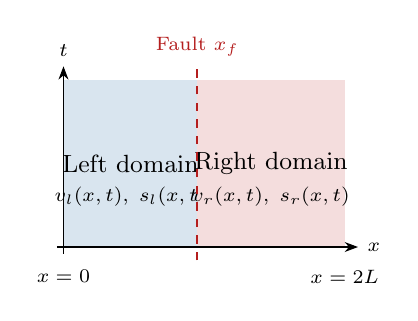
\begin{tikzpicture}[scale=0.85]
        % Left domain
        \fill[myblue!15] (0,0) rectangle (2.0,2.5);
        \node[font=\small] at (1.0,1.25) {Left domain};
        \node[font=\scriptsize] at (1.0,0.75) {$v_l(x,t),\; s_l(x,t)$};
        % Right domain
        \fill[myred!15] (2.0,0) rectangle (4.2,2.5);
        \node[font=\small] at (3.1,1.25) {Right domain};
        \node[font=\scriptsize] at (3.1,0.75) {$v_r(x,t),\; s_r(x,t)$};
        % Fault
        \draw[thick, myred, dashed] (2.0, -0.2) -- (2.0, 2.7)
              node[above, font=\scriptsize, text=myred] {Fault $x_f$};
        % Labels
        \node[font=\scriptsize, below] at (0, -0.2) {$x=0$};
        \node[font=\scriptsize, below] at (4.2, -0.2) {$x=2L$};
        % Arrows
        \draw[-{Stealth}] (-0.1,0) -- (4.4,0) node[right, font=\scriptsize] {$x$};
        \draw[-{Stealth}] (0,-0.1) -- (0,2.7) node[above, font=\scriptsize] {$t$};
      \end{tikzpicture}
    \end{column}
  \end{columns}
\end{frame}

\begin{frame}{Governing Equations: Elastic Wave System}
  \textbf{Velocity-stress form} (first-order hyperbolic):
  \begin{align}
    \frac{\partial v}{\partial t} &= \frac{1}{\rho}\frac{\partial s}{\partial x}
    && \text{(momentum)}\\[4pt]
    \frac{\partial s}{\partial t} &= \mu\,\frac{\partial v}{\partial x}
    && \text{(constitutive / Hooke's law)}
  \end{align}

  \vspace{6pt}
  \textbf{Spatial discretization}: \alert{Summation-by-Parts (SBP)} finite differences
  \begin{itemize}
    \item 4th-order interior, 2nd-order boundary stencils
    \item Satisfies a discrete energy estimate: $\frac{d}{dt}\|u_h\|_E^2 \le 0$
  \end{itemize}

  \vspace{6pt}
  \textbf{Boundary conditions}: \alert{Simultaneous-Approximation-Terms (SAT)}
  \begin{itemize}
    \item Fault interface: impose traction continuity + friction law weakly
    \item Absorbing (outflow) conditions at outer boundaries $x=0$, $x=2L$
  \end{itemize}
\end{frame}

\begin{frame}{Fault Friction: Slip-Weakening Law}
  \begin{columns}[T]
    \begin{column}{0.52\textwidth}
      Fault traction evolves with \textbf{total slip} $D$:
      \[
        \tau_{\rm SW}(D) = \sigma_n\Bigl[\alpha_s - (\alpha_s-\alpha_d)\min\!\Bigl(\tfrac{D}{D_c},1\Bigr)\Bigr]
      \]
      \begin{itemize}
        \item $\tau = \tau_0 + s_l(x_f,t)$ \quad (traction from left)
        \item Rupture nucleates when $\tau \ge \tau_{\rm SW}$
        \item Friction drops from $\alpha_s \sigma_n$ to $\alpha_d \sigma_n$ over distance $D_c$
      \end{itemize}
      \vspace{6pt}
      \textbf{Free parameters} (our operator input):
      \begin{center}
      \small
      \begin{tabular}{lll}
        \toprule
        Symbol & Description & Range \\
        \midrule
        $\tau_0$ & Background stress & [78, 88] MPa \\
        $\alpha_s$ & Static friction & [0.62, 0.74] \\
        $\alpha_d$ & Dynamic friction & [0.45, 0.55] \\
        $D_c$ & Critical slip dist. & [0.2, 0.8] m \\
        \bottomrule
      \end{tabular}
      \end{center}
    \end{column}
    \begin{column}{0.44\textwidth}
      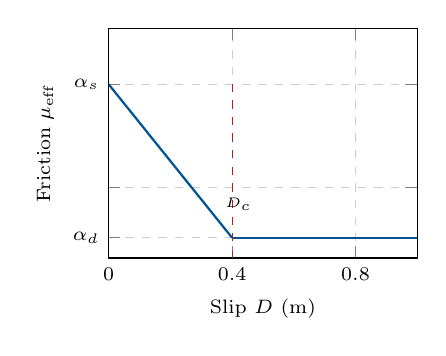
\begin{tikzpicture}
        \begin{axis}[
          width=5.5cm, height=4.5cm,
          xlabel={Slip $D$ (m)},
          ylabel={Friction $\mu_{\rm eff}$},
          xmin=0, xmax=1.0,
          ymin=0.42, ymax=0.76,
          xtick={0,0.4,0.8},
          ytick={0.45,0.525,0.677},
          yticklabels={$\alpha_d$, , $\alpha_s$},
          grid=major,
          grid style={dashed, gray!40},
          label style={font=\scriptsize},
          tick label style={font=\scriptsize},
        ]
          \addplot[thick, myblue, domain=0:0.4, samples=50]
            {0.677 - (0.677-0.45)*x/0.4};
          \addplot[thick, myblue, domain=0.4:1.0, samples=10]
            {0.45};
          \addplot[dashed, myred] coordinates {(0.4,0.42)(0.4,0.677)};
          \node[font=\tiny] at (axis cs: 0.42, 0.50) {$D_c$};
        \end{axis}
      \end{tikzpicture}
    \end{column}
  \end{columns}
\end{frame}

\begin{frame}{Time Integration \& Numba Acceleration}
  \begin{columns}[T]
    \begin{column}{0.50\textwidth}
      \textbf{Time integration}
      \begin{itemize}
        \item Classical 4th-order Runge-Kutta (RK4)
        \item CFL-stable time step: $\Delta t = \text{CFL}\cdot\Delta x / c_s$
        \item $n_x = 501$ grid points, $n_t \approx 577$ steps
        \item Fields stored every \texttt{iplot} steps
      \end{itemize}
      \vspace{8pt}
      \textbf{Numba JIT acceleration}
      \begin{itemize}
        \item All kernels: \texttt{@njit(parallel=True)}
        \item Pure-Python serial: \textbf{160 s/run}
        \item Numba (1 thread): \textbf{0.086 s/run}
        \item \alert{$\bm{1868\times}$ speedup}
        \item Multi-thread: \textit{negative} scaling — thread overhead $>$ compute at $n_x=501$
      \end{itemize}
    \end{column}
    \begin{column}{0.46\textwidth}
      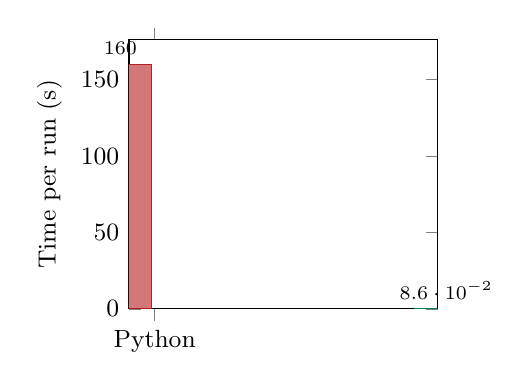
\begin{tikzpicture}
        \begin{axis}[
          ybar,
          width=5.5cm, height=5.0cm,
          bar width=0.8cm,
          ylabel={Time per run (s)},
          symbolic x coords={Python, Numba},
          xtick=data,
          ymin=0,
          nodes near coords,
          nodes near coords align={vertical},
          label style={font=\small},
          tick label style={font=\small},
          every node near coord/.append style={font=\scriptsize},
        ]
          \addplot[fill=myred!60, draw=myred] coordinates {(Python,160)};
          \addplot[fill=mygreen!70, draw=mygreen] coordinates {(Numba,0.086)};
        \end{axis}
      \end{tikzpicture}
      \vspace{4pt}
      \centering\small\textcolor{mygreen}{\textbf{1868$\times$ faster than Python serial}}
    \end{column}
  \end{columns}
\end{frame}

% ══════════════════════════════════════════════════════════════════════════════
\section{FNO Architecture}
% ══════════════════════════════════════════════════════════════════════════════

\begin{frame}{Operator Learning: Problem Formulation}
  \textbf{Goal}: Learn the parameter-to-solution operator
  \[
    \G\;:\; \bm{p} = (\tau_0,\,\alpha_s,\,\alpha_d,\,D_c)
    \;\longmapsto\;
    \bigl(\vl(x,t),\;\ssl(x,t),\;\vr(x,t),\;\ssr(x,t)\bigr)
  \]

  \vspace{6pt}
  \begin{columns}[T]
    \begin{column}{0.48\textwidth}
      \textbf{Why not a standard neural network?}
      \begin{itemize}
        \item Output is a \textit{function} on a 2D grid $(x,t) \in [0,L]\times[0,T]$
        \item $64 \times 64 \times 4 = 16{,}384$ output values
        \item Solution structure is \textit{non-local} (wave propagation)
        \item Standard CNN/MLP won't generalize across resolutions
      \end{itemize}
    \end{column}
    \begin{column}{0.48\textwidth}
      \textbf{Why Fourier Neural Operators (FNO)?}
      \begin{itemize}
        \item Learns \textit{integral operators} in Fourier space
        \item Resolution-invariant by design
        \item Exact global basis functions (Fourier modes)
        \item State-of-the-art on PDE solution operators
        \item Efficient: $\mathcal{O}(n \log n)$ via FFT
      \end{itemize}
    \end{column}
  \end{columns}
\end{frame}

\begin{frame}{FNO-2D Architecture}
  \begin{center}
  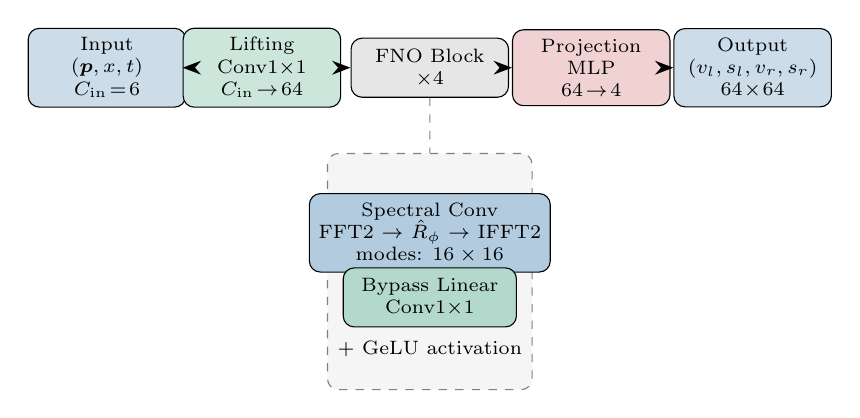
\begin{tikzpicture}[scale=0.82,
      block/.style={draw, rounded corners, fill=#1, minimum width=2.0cm,
                    minimum height=0.75cm, align=center, font=\scriptsize},
      arr/.style={-{Stealth}, thick}
  ]
    \node[block=myblue!20] (inp) at (0,0)
      {Input\\$(\bm{p}, x, t)$\\$C_{\rm in}\!=\!6$};

    \node[block=mygreen!20] (lift) at (2.4,0)
      {Lifting\\Conv1$\times$1\\$C_{\rm in}\!\to\!64$};

    \node[block=mygray] (fno1) at (5.0,0)
      {FNO Block\\$\times 4$};

    \node[block=myred!20] (proj) at (7.5,0)
      {Projection\\MLP\\$64\!\to\!4$};

    \node[block=myblue!20] (out) at (10.0,0)
      {Output\\$(\vl,\ssl,\vr,\ssr)$\\$64\!\times\!64$};

    \draw[arr] (inp) -- (lift);
    \draw[arr] (lift) -- (fno1);
    \draw[arr] (fno1) -- (proj);
    \draw[arr] (proj) -- (out);

    % FNO Block detail box
    \node[draw=gray, dashed, rounded corners, fill=mygray!40,
          minimum width=2.6cm, minimum height=3.0cm, below=0.7cm of fno1] (detail) {};
    \node[block=myblue!30, minimum width=2.2cm] at ([yshift=0.6cm]detail.center)
      (spec) {Spectral Conv\\FFT2 $\to$ $\hat{R}_\phi$ $\to$ IFFT2\\modes: $16\times16$};
    \node[block=mygreen!30, minimum width=2.2cm] at ([yshift=-0.4cm]detail.center)
      (lin) {Bypass Linear\\Conv1$\times$1};
    \node[font=\scriptsize, below=0.05cm of lin] {$+$ GeLU activation};

    \draw[dashed, gray] (fno1.south) -- (detail.north);
  \end{tikzpicture}
  \end{center}

  \vspace{4pt}
  \begin{columns}
    \begin{column}{0.33\textwidth}
      \centering\small
      \textbf{Input:} $(B, 6, 64, 64)$\\
      params $+$ $(x,t)$ coords
    \end{column}
    \begin{column}{0.33\textwidth}
      \centering\small
      \textbf{FNO Block}: spectral conv\\
      $+$ pointwise linear $+$ GeLU
    \end{column}
    \begin{column}{0.33\textwidth}
      \centering\small
      \textbf{Total params:}\\
      \alert{\textbf{8.4 million}}
    \end{column}
  \end{columns}
\end{frame}

\begin{frame}{Spectral Convolution Layer}
  \textbf{Key idea}: replace spatial convolution with a \textit{global} Fourier integral operator
  \begin{align}
    (\mathcal{K}_\phi\, u)(x,t)
    &= \mathcal{F}^{-1}\!\Bigl[\hat{R}_\phi(k_x, k_t)\cdot \mathcal{F}[u](k_x, k_t)\Bigr](x,t)
  \end{align}

  \begin{columns}[T]
    \begin{column}{0.50\textwidth}
      \textbf{Implementation}
      \begin{enumerate}
        \item \textbf{FFT2} the input: $\hat{u} = \mathcal{F}[u]$
        \item Multiply by complex weights $\hat{R}_\phi$ for the first $k_{\rm max}$ modes
        \item \textbf{IFFT2} back to physical space
        \item Add pointwise linear bypass
      \end{enumerate}
      \vspace{4pt}
      $\Rightarrow$ Modes beyond $k_{\rm max}$ are \textit{truncated} (low-pass filter)
    \end{column}
    \begin{column}{0.46\textwidth}
      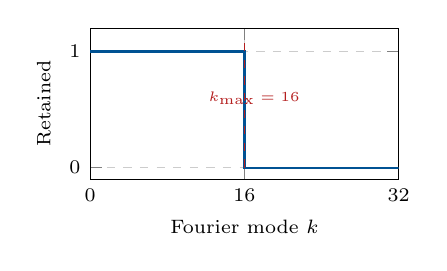
\begin{tikzpicture}
        \begin{axis}[
          width=5.5cm, height=3.5cm,
          xlabel={Fourier mode $k$},
          ylabel={Retained},
          xmin=0, xmax=32,
          ymin=-0.1, ymax=1.2,
          ytick={0,1},
          yticklabels={0,1},
          xtick={0,16,32},
          grid=major,
          grid style={dashed, gray!40},
          label style={font=\scriptsize},
          tick label style={font=\scriptsize},
        ]
          \addplot[thick, myblue, const plot]
            coordinates {(0,1)(16,0)(32,0)};
          \addplot[dashed, myred] coordinates {(16,0)(16,1.1)};
          \node[font=\tiny, text=myred] at (axis cs:17,0.6) {$k_{\max}=16$};
        \end{axis}
      \end{tikzpicture}
    \end{column}
  \end{columns}
\end{frame}

% ══════════════════════════════════════════════════════════════════════════════
\section{Dataset \& Training}
% ══════════════════════════════════════════════════════════════════════════════

\begin{frame}{Dataset Generation via Latin Hypercube Sampling}
  \begin{columns}[T]
    \begin{column}{0.50\textwidth}
      \textbf{Sampling strategy}
      \begin{itemize}
        \item Latin Hypercube Sampling (LHS) over 4D parameter space
        \item LHS ensures uniform coverage — no clustering
        \item Validity constraints enforced:
          \begin{itemize}\small
            \item $\alpha_d < \alpha_s$ (velocity-weakening)
            \item $\tau_0 > \alpha_s\sigma_n$ (nucleation condition)
          \end{itemize}
      \end{itemize}
      \vspace{6pt}
      \textbf{Dataset splits}
      \begin{center}
      \small
      \begin{tabular}{lrr}
        \toprule
        Split & Samples & Time \\
        \midrule
        Train & 200 & $\sim$46 s \\
        Val   &  50 & $\sim$12 s \\
        Test  &  50 & $\sim$12 s \\
        \midrule
        Total & 300 & $\sim$70 s \\
        \bottomrule
      \end{tabular}
      \end{center}
    \end{column}
    \begin{column}{0.46\textwidth}
      \textbf{Output per sample}\\[4pt]
      \small
      Downsample simulator output to $64\times64$ grid:
      \begin{itemize}
        \item $v_l(x,t)$, $s_l(x,t)$ \hfill left domain
        \item $v_r(x,t)$, $s_r(x,t)$ \hfill right domain
        \item Fault time series: slip, slip-rate, traction
      \end{itemize}
      \vspace{6pt}
      \textbf{Normalization}
      \begin{itemize}
        \item Parameters: zero-mean unit-std (fit on train)
        \item Fields: channel-wise zero-mean unit-std
        \item Applied consistently to val/test
      \end{itemize}
    \end{column}
  \end{columns}
\end{frame}

\begin{frame}{Training Setup}
  \begin{columns}[T]
    \begin{column}{0.50\textwidth}
      \textbf{Loss function (supervised)}
      \[
        \loss_{\rm data} = \frac{1}{N}\sum_{i=1}^N
        \frac{\|\G(\bm{p}_i) - u_i\|_2}{\|u_i\|_2}
      \]
      Relative $L^2$: scale-invariant, treats all fields equally.

      \vspace{8pt}
      \textbf{Optimizer}: AdamW
      \begin{itemize}
        \item $\ell_r = 10^{-3}$, weight decay $= 10^{-4}$
        \item Gradient clip at norm $= 1.0$
      \end{itemize}

      \vspace{6pt}
      \textbf{LR Schedule}: cosine decay
      \begin{itemize}
        \item Linear warmup for first 10 epochs
        \item Cosine anneal: $10^{-3} \to 0$ over 200 epochs
      \end{itemize}
    \end{column}
    \begin{column}{0.46\textwidth}
      \textbf{Hardware \& settings}
      \begin{itemize}
        \item CPU-only (no GPU on this node)
        \item Batch size: 16
        \item Epochs: 200
        \item $\approx$14.4 s/epoch on CPU
        \item Total training time: $\approx$48 min
      \end{itemize}

      \vspace{8pt}
      \textbf{Future: PINO loss}
      \[
        \loss = \loss_{\rm data}
               + \lambda_{\rm PDE}\,\loss_{\rm PDE}
               + \lambda_{\rm BC}\,\loss_{\rm BC}
      \]
      \begin{itemize}
        \item Currently: $\lambda_{\rm PDE}=0$ (baseline)
        \item PDE residuals computed \textit{exactly} in Fourier space
      \end{itemize}
    \end{column}
  \end{columns}
\end{frame}

% ══════════════════════════════════════════════════════════════════════════════
\section{Results}
% ══════════════════════════════════════════════════════════════════════════════

\begin{frame}{Training Convergence}
  \begin{columns}[T]
    \begin{column}{0.50\textwidth}
      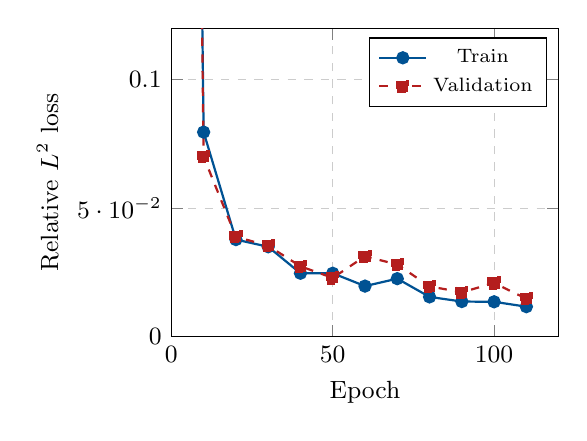
\begin{tikzpicture}
        \begin{axis}[
          width=6.5cm, height=5.5cm,
          xlabel={Epoch},
          ylabel={Relative $L^2$ loss},
          xmin=0, xmax=120,
          ymin=0, ymax=0.12,
          legend pos=north east,
          legend style={font=\scriptsize},
          grid=major,
          grid style={dashed, gray!40},
          label style={font=\small},
          tick label style={font=\small},
        ]
          % Train loss
          \addplot[thick, myblue, mark=*, mark size=2pt]
            coordinates {
              (1,1.001)(10,0.0796)(20,0.0378)(30,0.0350)
              (40,0.0247)(50,0.0247)(60,0.0197)(70,0.0226)
              (80,0.0155)(90,0.0137)(100,0.0136)(110,0.0117)
            };
          % Val loss
          \addplot[thick, myred, dashed, mark=square*, mark size=2pt]
            coordinates {
              (1,1.001)(10,0.0700)(20,0.0389)(30,0.0354)
              (40,0.0274)(50,0.0229)(60,0.0313)(70,0.0281)
              (80,0.0196)(90,0.0173)(100,0.0209)(110,0.0148)
            };
          \legend{Train, Validation}
        \end{axis}
      \end{tikzpicture}
    \end{column}
    \begin{column}{0.46\textwidth}
      \textbf{Key observations}
      \begin{itemize}
        \item Epoch 1 $\to$ 10: \textbf{92\% drop} in loss\\
          (network learns dominant modes quickly)
        \item Train $\approx$ Val $\Rightarrow$ no overfitting
        \item \textbf{Best val loss: 0.0148}\\
          at epoch 110 ($\approx$1.5\% rel. error)
        \item Still improving — training ongoing
      \end{itemize}

      \vspace{8pt}
      \begin{block}{Summary so far}
        \small
        FNO achieves $<$2\% relative $L^2$ error on all 4 fields after 110 epochs of CPU training.
      \end{block}
    \end{column}
  \end{columns}
\end{frame}

\begin{frame}{Expected Speedup at Inference}
  \begin{columns}[T]
    \begin{column}{0.50\textwidth}
      \begin{tikzpicture}
        \begin{axis}[
          xbar,
          width=6.0cm, height=4.5cm,
          bar width=0.5cm,
          xlabel={Time per evaluation (ms)},
          symbolic y coords={Python serial, Numba (np=1), FNO (CPU), FNO (GPU)},
          ytick=data,
          xmin=0,
          nodes near coords,
          nodes near coords align={horizontal},
          label style={font=\small},
          tick label style={font=\scriptsize},
          every node near coord/.append style={font=\scriptsize},
          xmax=200000,
        ]
          \addplot[fill=myred!60] coordinates
            {(160000,{Python serial})};
          \addplot[fill=myblue!60] coordinates
            {(86,{Numba (np=1)})};
          \addplot[fill=mygreen!60] coordinates
            {(5,{FNO (CPU)})};
          \addplot[fill=mygreen!90] coordinates
            {(0.5,{FNO (GPU)})};
        \end{axis}
      \end{tikzpicture}
    \end{column}
    \begin{column}{0.46\textwidth}
      \small
      \begin{tabular}{lrr}
        \toprule
        Method & Time & Speedup \\
        \midrule
        Python serial   & 160 s    & $1\times$ \\
        Numba (np=1)    & 86 ms    & $1{,}868\times$ \\
        FNO (CPU, est.) & $\sim$5 ms  & $\sim$$32{,}000\times$ \\
        FNO (GPU, proj.)& $<$1 ms  & $>$$10^5\times$ \\
        \bottomrule
      \end{tabular}

      \vspace{8pt}
      \textbf{Key advantage}:\\
      FNO inference $\approx$ matrix multiply + FFT — highly parallelizable.

      \vspace{4pt}
      Simulator must march forward in time; FNO predicts the \textit{entire} space-time solution in one forward pass.
    \end{column}
  \end{columns}
\end{frame}

% ══════════════════════════════════════════════════════════════════════════════
\section{PINO Extension}
% ══════════════════════════════════════════════════════════════════════════════

\begin{frame}{Physics-Informed Extension (PINO)}
  \textbf{Idea}: supplement data loss with PDE residuals — enforce governing equations in the prediction.

  \vspace{6pt}
  \textbf{PDE residuals} (evaluated \textit{exactly} in Fourier space):
  \[
    \loss_{\rm PDE} = \underbrace{\left\|\partial_t \vl^\theta
                      - \tfrac{1}{\rho}\partial_x \ssl^\theta\right\|^2}_{\text{momentum}}
                    + \underbrace{\left\|\partial_t \ssl^\theta
                      - \mu\,\partial_x \vl^\theta\right\|^2}_{\text{constitutive}}
                    + \; \text{(right domain)}
  \]

  Derivatives via FFT: $\hat{\partial}_x u = ik_x\hat{u}$, \quad $\hat{\partial}_t u = i\omega\hat{u}$

  \vspace{6pt}
  \textbf{Fault boundary loss} (SW friction residual):
  \[
    \loss_{\rm BC} = \bigl\|\tau^\theta - \tau_{\rm SW}(D^\theta, \bm{p})\bigr\|^2
                   + \bigl\|s_l^\theta(x_f) + s_r^\theta(x_f)\bigr\|^2
  \]

  \vspace{4pt}
  \begin{alertblock}{PINO advantage over PINN}
    \small
    PINN uses finite differences for derivatives (inaccurate, slow).
    PINO uses FFT derivatives — \textit{spectrally accurate} and fast.
    No spatial collocation points needed.
  \end{alertblock}
\end{frame}

% ══════════════════════════════════════════════════════════════════════════════
\section{Conclusions \& Future Work}
% ══════════════════════════════════════════════════════════════════════════════

\begin{frame}{Conclusions}
  \begin{columns}[T]
    \begin{column}{0.50\textwidth}
      \textbf{What we built}
      \begin{itemize}
        \item High-performance 1D rupture simulator\\(Numba, 1868$\times$ speedup)
        \item FNO-2D surrogate: maps 4 scalar parameters to full space-time fields
        \item PINO extension: PDE + BC residual losses in Fourier space
        \item Complete pipeline: LHS data generation $\to$ training $\to$ evaluation
      \end{itemize}
    \end{column}
    \begin{column}{0.46\textwidth}
      \textbf{Results (POC)}
      \begin{itemize}
        \item 300 training samples generated in $<$2 min
        \item Val loss $\approx$\textbf{1.5\%} rel. $L^2$ error in 110 epochs
        \item No overfitting (train $\approx$ val)
        \item Expected speedup: $\sim$$10^4$--$10^5\times$ vs. simulator
        \item 8.4M parameter model trains in $<$1 hr on CPU
      \end{itemize}
    \end{column}
  \end{columns}

  \vspace{10pt}
  \textbf{Future work}
  \begin{itemize}
    \item Enable PINO loss ($\lambda_{\rm PDE} > 0$) and measure physics consistency improvement
    \item Scale to 2000 samples, expand to 6-parameter space (add $\sigma_n$, $c_s$)
    \item GPU training for sub-millisecond inference
    \item Extend to 3D rupture dynamics (WaveQLab3D interface)
  \end{itemize}
\end{frame}

\begin{frame}{Thank You}
  \begin{center}
    {\Large \textbf{Questions?}}\\[16pt]

    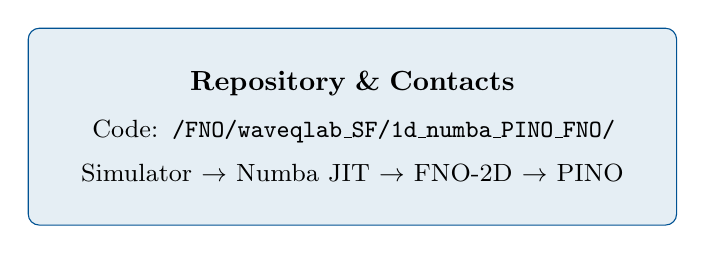
\begin{tikzpicture}
      \node[draw=myblue, fill=myblue!10, rounded corners, minimum width=8cm,
            minimum height=2.5cm, text width=8cm, align=center] {
        \textbf{Repository \& Contacts}\\[6pt]
        \small
        Code: \texttt{/FNO/waveqlab\_SF/1d\_numba\_PINO\_FNO/}\\[4pt]
        Simulator $\to$ Numba JIT $\to$ FNO-2D $\to$ PINO
      };
    \end{tikzpicture}

    \vspace{12pt}
    \begin{tabular}{ll}
      \toprule
      \textbf{Simulator}   & SBP-SAT $+$ RK4, SW friction, Numba \\
      \textbf{Surrogate}   & FNO-2D, 8.4M params, 64$\times$64 grid \\
      \textbf{Current acc.}& $\sim$1.5\% relative $L^2$ (110 epochs) \\
      \textbf{Speedup}     & $\sim$$10^4\times$ (CPU), $>$$10^5\times$ (GPU) \\
      \bottomrule
    \end{tabular}
  \end{center}
\end{frame}

% ══════════════════════════════════════════════════════════════════════════════
% Appendix
% ══════════════════════════════════════════════════════════════════════════════
\appendix
\section*{Backup Slides}

\begin{frame}{SBP-SAT Discretization Details}
  \textbf{SBP derivative operator}: $D_1 = H^{-1} Q$
  \begin{itemize}
    \item $H$ — positive definite diagonal norm matrix
    \item $Q$ — nearly skew-symmetric: $Q + Q^T = \text{diag}(-1,0,\ldots,0,1)$
    \item Guarantees: $u^T H D_1 u = $ boundary terms only (mimics integration by parts)
  \end{itemize}

  \vspace{8pt}
  \textbf{SAT penalty for fault interface}: At $x = x_f$:
  \[
    \text{SAT} = H^{-1}\bigl[\tau - \tau_{\rm SW}(D)\bigr]\,\mathbf{e}_{n_x}
  \]
  where $\mathbf{e}_{n_x}$ is the unit vector at the fault node. This imposes the friction law weakly without modifying the interior stencil.

  \vspace{4pt}
  \textbf{Energy stability}: The SBP-SAT combination satisfies
  \[
    \frac{d}{dt}\|u_h\|_{H}^2 = \text{boundary terms} \le 0
  \]
  ensuring the scheme is non-growing (analogous to the continuous energy estimate).
\end{frame}

\begin{frame}{Parameter Space \& Validity Constraints}
  \begin{columns}[T]
    \begin{column}{0.50\textwidth}
      \textbf{All parameters}
      \begin{center}
      \small
      \begin{tabular}{llll}
        \toprule
        Symbol & Description & Range & Fixed? \\
        \midrule
        $\tau_0$    & Background stress & [78, 88] MPa & No \\
        $\alpha_s$  & Static friction   & [0.62, 0.74] & No \\
        $\alpha_d$  & Dynamic friction  & [0.45, 0.55] & No \\
        $D_c$       & Critical slip     & [0.2, 0.8] m & No \\
        $\sigma_n$  & Normal stress     & 120 MPa      & Yes \\
        $c_s$       & Shear wave speed  & 3.464 km/s   & Yes \\
        $\rho$      & Density           & 2670 kg/m$^3$& Yes \\
        \bottomrule
      \end{tabular}
      \end{center}
    \end{column}
    \begin{column}{0.46\textwidth}
      \textbf{Validity constraints}
      \begin{enumerate}
        \item \textbf{Velocity-weakening}:\\
          $\alpha_d < \alpha_s$\\
          (friction must decrease with slip)
        \item \textbf{Nucleation condition}:\\
          $\tau_0 > \alpha_s \sigma_n$\\
          (background stress must exceed\\ peak static friction strength)
      \end{enumerate}
      \vspace{6pt}
      LHS oversamples by $3\times$ and rejects invalid draws. All 300 samples generated without issues.
    \end{column}
  \end{columns}
\end{frame}

\end{document}
